\documentclass[]{../../../../tex/classes/styledArticle}
\usepackage{../../../../tex/packages/hebrewSupport}
\usepackage{../../../../tex/packages/mathShortcuts}
\usepackage{../../../../tex/packages/theoremsSupport}

\usetikzlibrary{graphs}
\usepackage{listings}
\lstset{
	language=Python,
	numbers=left,
	breaklines,
	basicstyle=\ttfamily,
	commentstyle=\color{gray},
	prebreak=\textrightarrow,
}

\author{שחר פרץ}
\title{אלגוריתמים $\sim$ \textit{הרצאה 7}}
\begin{document}
	\maketitle
	\textbf{מרצה: }עמית ווינשטיין
	
	\defi{אומרים ש\textit{רשת זרימה} היא גרף מכוון שכל קשת בגרף מייצגת מעבר ישיר בין שני צמתים, ויש לה קיבול מקסימלי. }
	
	\begin{center}
		\sen
		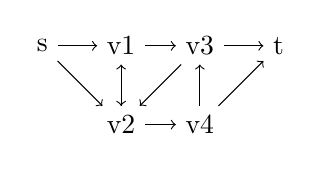
\begin{tikzpicture}
			\graph {s -> {v1 -> v3, v2 -> v4} -> t, v4 -> v3, v2 -> v1, v1 -> v2, v3 -> v2};
		\end{tikzpicture}
		\she
	\end{center}
	וערמה של משקלים/קיבולות שאין לי מושג איך להעתיק לתוך הגרף. 
	\begin{itemize}
		\item מעניינים אותנו רק צמתי שיש מסלול מ־$s$ אליהם, ויש מהם מסלול ל־$t$. בפרט, צריך שיהיה מסלול מ־$s$ ל־$t$. בהינתן שהצטמצמנו לצמתים רלוונטיים, הגרף קשיר במובן הלא מכוון שלו, ולכן $\sof E \ge \sof V - 1$. 
		\item מטרה: למקסם את כמות הזרימה/חומר שעובר מ־$s$ ל־$t$. 
		\item לא נזרים על קשת יותר מהקיבולת שלה
		\item נרצה שכל החומר שיוצא מ־$s$ יגיע ל־$t$. זו דרישה לוקאלית (כמות החומר שנכנסת מקודקוד מסוים, שווה לכמות החומר שיוצאת). ''חוק שימור החומר``. 
	\end{itemize}
	
	רשת זרימה, זה גרף $G = (V, E)$ ופונקציית קיבולת $c \co E \to \R^{+}$, כך ש־$c(u, v) > 0$. קשת עם קיבולת אפס פשוט לא תופיע ברשת/גרף. מניחים שכל צומת נגיש מ־$s$ ויש מסלול ל־$t$. ההגדרה של \textit{זרימה} (לא קשת זרימה) היא פונקציה $f \co V \times V \to \R$ המתארת כמה זרימה ישירה יש בין כל זוג קודקודים (יתאפס בין קודקודים שאין בינהם קשת). 
	
	\textbf{תכונות: }
	\begin{itemize}
		\item \textit{אילוץ הקיבול: }$f(u, v) \le c(u, v)$. אם $(u, v)$ לא קשת, נניח $c(u, v) = 0$. 
		\item \textit{אנטי־סימטריה: }$f(u, v) = -f(v, u)$. 
		\item \textit{חוק שימור הזרימה: }לכל $u \neq s, t$, מתקיים $\sum_{v \in V} f(u, v) = 0$ (כלומר סכום החומר שנכנס=סכום החומר שיוצא). 
	\end{itemize}
	מהתכונות האחרות, נובע ש־$f(u, u) = 0$, ואם $u, v$ אינם שכנים אז $f(u, v) = 0$. 
	נגדיר את ערך הזרימה להיות: 
	\noti{\hfil $\disty \sof f := \sum_{v \in V} f(s, v) \seq \sum_{v \in V} f(v, t)$}
	את השוויון המסומן ב־$\seq$ נוכיח אח''כ. 
	
	\defi{הרחבת ההגדרה: עבור קבוצות $X, Y$ של צמתים נוכל להגדיר: 
		\[ f(X, Y) := \sum_{\mathclap{u \in X, v \in Y}}f(u, v) \quad \quad c(x, y) = \sum_{\mathclap{u \in X, v \in Y}} c(u, v) \]}
	
	הזרימה המוכללת מקיימת את מה שנצפה ממנה: 
	\begin{itemize}
		\item $f(X, Y) = -f(Y, X)$ (הוכחה באמצעות דיסטרבוטיביות)
		\item $f(X, X) = 0$ (הוכחה באמצעות קומטטיביות והופכי לחיבור)
		\item אם $X, Y$ זרות, אזי $f(X \uplus Y, Z) = f(X, Z) + f(Y, Z)$. (הוכחה באמצעות אסוציאטיביות)
	\end{itemize}
	יש לנו כמה טענות ''פחות טרוויאליות``
	\lem{
	\[ \sof f = \sum_{v \in V} f(s, v) = f(\{s\}, V) = f(V, \{s\}) = \sum_{v \in V}f(t, v) \]}
	\begin{proof}
		קל לראות ש־$V = \{s\} \uplus (V \setminus \{s\})$. מכאן ש־: 
		\begin{multline*}
			0 = f(v, v) = f(\{s\}, V) + f(V \setminus \{s\}, V) 
			\\ \implies f(\{s\}, V) = -f(V \setminus \{s\}, V) = f(V, V \setminus \{s\}) = f(V, V \setminus\{s, t\}) + f(V, \{t\}) \seq f(V, \{t\})
		\end{multline*}
		השוויון המסומן ב־$\seq$ תלוי בכך ש־$f(V, V \setminus \{s, t\}) = 0$. זה נכון כי מאסוציאטיביות סכומים ומחוק שימור הזרימה נקבל: 
		\[ f(V, V \setminus \{s, t\}) = \sum_{\mathclap{u \in V, v \in V \setminus \{s, t\}}} f(u, v) = \sum_{v \in V \setminus \{s, t\}} \underbrace{\sum_{u \in V} f(u, v)}_{0} = 0 \]\envendproof
	\end{proof}
	
	
	עכשיו יש לנו את כל הכלים למציאת זרימה מקסימלית. 
	
	האלגוריתם ברעיון כללי: 
	\begin{center}
		\sen
		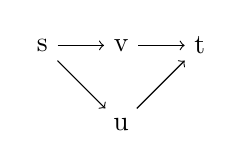
\begin{tikzpicture}
			\graph {s -> {v, u} -> t};
		\end{tikzpicture}
		$\implies$
		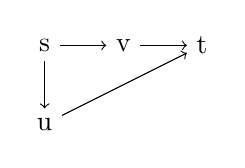
\begin{tikzpicture}
			\graph {s -> v -> t, u <- s, u -> t,};
		\end{tikzpicture}
		$\implies$
		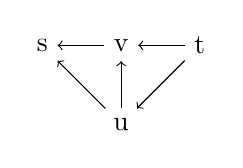
\begin{tikzpicture}
			\graph {s <- {v, u} <- t, u -> v};
		\end{tikzpicture}
		\she
	\end{center}
	
			(כאשר הקשתות ממשקלים בגודל $1$). 
	
	\textbf{הרעיון: }נחפש מסלול מ־$s$ ל־$t$. נזרים לאורכו לפי הקיבול המינימלי של קשת עליו. נוכל לעדכן את הזרימה $f$ בצורה תקינה. לכל $u, v$ שאינם שכנים על המסלול, $f(u, v)$ נשאר ללא שינוי. עבור $u, v$ כך ש־$(u, v)$ קשת במסלול, $d(u ,v)$ תוגדר לפי כמה שהזרמנו. אם $v, u$ קשת סמלול, נחסר מ־$f(u, v)$ את הערך שהזרמנו. 
	
	בצעד הבא נעבור על הרשת השיעורית  (residual network) המורכבת מהקשתות המקרויות של הגרף והאנטי־קשתות, כאשר $c_f(u, v) = c(u, v) - f(u, v)$ (קיבול שיורי של רשת $(u, v)$ תחת זרימה $f$). קשת נקראת \textit{רוויה} אם הקיבול השיורי של הוא $0$ (ואז היא לא בקשת). נעצור כאשר אין מסלול מ־$s$ ל־$t$ ברשת השיורית. 
	
	
	אם הזרמנו $c_{\min}$ הקיבול המינימל ילאורך המסלול, אז נשה: 
	\[ f'(u, v) =  \begin{cases}
		f(u, v) + c_{\min} & (u, v) \in P \\
		f(u, v) - c_{\min} & (v, u) \in P\\
		u \neq v & \text{נניח שהמסלול פשוט}
	\end{cases} \]
	
	\lem{$f'$ גם היא זרימה תקינה אם $f$ תקינה. }
	\lem{ערך הזרימה משתפר ממש בכל איטרציה, כלומר $\sof {f'} > \sof f$. }
	
	שאלות להפסקה: 
	\begin{itemize}
		\item האם השיטה הזו תמיד עוצרת? \textbf{לא$^{\text{*}}$\!. }אבל החדשות הטובות הן שזה לא עוצר במקרה שבו אפשר תמיד לשפר את הזרימה, לאין שיעור. מכיוון שיש חסם עליון לגבי הזרימה, ומכאן שהקיבולים במקרה זה לא שלמים, ומשום שבמקרה של מספרים אי רציונליים תמיד אפשר לכפול במכנה המשותף ולקבל קיבולים שלמים – תנאי הכרחי לרשתות כאלו הוא שיהיו קיבולים אי רציונליים. אז לא באמת אכפת לנו מזה (כי אין באמת מספרים אי־רציונליים במחשב). 
		\item אם וכאשר היא עוצרת, מה הסיבוכיות של הסיפור הזה (האם יש חסם טוב לכמה זמן לקח לה לעצור). \textbf{רע. }יותר גרוע מאקספוננציאלי בכמות הקשתות. זה לא מפתיע בהתחשב בזה שבאי־רציונליים החרא הזה לא מסתיים לעולם. גם תחת ההנחה של קיבולים שלמים, חסם עליון טרוויאלי הוא סכום הקיבולים, חסם טרוויאלי קצת יותר הדוק זה ערך הזרימה המקסימלית. אבל אפשר להראות שחסם הדוק אפשרי הוא כמות הקיבולים (מבחינת הערך שלהם, לא הקשתות) שנכנסים ל־$t$ או כמות הקיבולים שיוצאים מ־$s$. 
		
		נסכם: בעבור זרימה על קיבולים שלמים, כמות האיטרציות חסומה ע''י $\sof{f^{^*}}$ כאשר $f^{*}$ היא הזרימה המקסימלית (וכמובן $\sof{f^*} \le c(\{s, V\})$). 
		\item בהנחה שהיא עוצרת, האם היא הגיעה לזרימה המקסימלית. \textbf{כן. }סוףסוף משהו חיובי. (''הוכחה משמעותית``)
	\end{itemize}
	
	זהו הרעיון הכללי מאחורי השיטה של Ford-Folkerson. בדיוק כמו באלגוריתם האחר של Ford, נצטרך לעשות קצת עבודה כדי להפוך אותו ליותר מועיל. 
	
	קל לראות (באמת קל לראות. אין לי מושג מה קורה בהרצאה והפלצתי את הטענה הזו) שבהינתן קבוצה $S$ של קודקודים דרכם כל מסלול מ־$s$ ל־$t$ חייב לעבור בהם, מתקיים ש־$\sof{f^*} \le \sum_{s \in S, u \notin S} c(s, u)$. 
	אם ניקח את האינפימום (אני מתכוון, מינימום) של ה־$S$־ים האפשריים, נקבל \textbf{בדיוק} את הזרימה המקסימלית. זה לעומת הטענה הקודמת, לא טרוויאלי בשיט. למשפט זה קוראים max-flow min-cut. נפרמל קצת את זה. 
	
	\defi{נגדיר \textit{חתך} $S, T$ כך ש־$S \cup T = V$, וכן $S \cap T = \varnothing \land s \in S, t \in T$. נגדיר את קיבול החתך להיות (סופר קשתות בלבד): 
	\[ c(S, T) = \sum_{\mathclap{v \in S, u \in T}}c(v, u) \]
	וזרימת החתך (סופר קשתות ואנטי־קשתות):
	\[ f(S, T) = \sum_{\mathclap{v \in S, u \in T}}f(v, u) \]}
	\theo{לכל חתך $S, T$ מתקיים $f(S, T) = \sof f$}\begin{proof}
		\[ f(S, T) \seq f(S, V) = \underbrace{f(\{s\}, V)}_{\sof f} + \underbrace{f(S \setminus \{s\}, V)}_{0} \]
		כאשר $\seq$ מתקיים כי: 
		\[ f(S, T) + \smash{\overbrace{f(S, S)}^{0}} = f(S, V) \]
	\end{proof}
	\theo{לכל חתך $S, T$ מתקיים $f(S, T) \le c(S, T)$. }
	\cola{בפרט, $\sof{f^{^*}} \le c(S, T)$ לכל חתך $S, T$. בפרט היא קטנה מהמינימום על פני כל החתכים. }
	\begin{Theorem}[Max Flow Min Cut]
		הטענות הבאות שקולות: 
		\begin{itemize}
			\item $f$ זרימה מקסימלית
			\item הרשת השיורית $G_f$ לא מכילה מסלול משפר מ־$s$ ל־$t$. 
			\item $\sof f = c(S, T)$ בעבור חתך כלשהו. 
		\end{itemize}
	\end{Theorem}
	\begin{proof}\,
		\begin{itemize}
			\item[$1 \implies 2$]אחרת היינו משפרים
			\item[$3 \implies 1$]כל חתך הוא חסם עליון, ולכן $f$ מקסימלית. 
			\item[$2 \implies 3$]נגדיר את $S$ להיות כל הקודקודים שנגישים מ־$S$ ב־$G_f$. $T = V \setminus S$. ברור ש־$s \in S, t \in T$ כי אין מסלול משפר. כל הקשתות בחתך $(S, T)$ רוויות שכן לא ניתן להגיע מ־$s$ לקודקודים ב־$T$. 
			
			לכן לכל $u \in S, v \in V$ מתקיים $f(u, v) = c(u, v)$. מצד שני, 
			
			\hfil $\disty \sof f = f(S, T) = \sum_{u \in S, v \in T} f(u, v) = \sum_{u \in S, v \in T}c(u, v) = c(S, T)$
			
			וסיימנו. 
		\end{itemize}
	\end{proof}
	\cola{כש־FF עוצר, הוא מצא זרימה מקסימלית. }
	
	פורד המסכן לא טורח להגיד לנו איך הוא בוחר מסלולים. האלגוריתם של Admonds-Kare עושה שינוי קטן: מבין המסלולים, נבחר תמיד מסלול משפר קצר ביותר. 
	
	\theo{ב־EK, לכל צומת $v$ הערך $\dg_f(s, v)$ עולה חלש במהלך הריצה. }
	($\dg_f$ הוא המרחק ברשת השיורית $G_f$)
	\begin{proof}
		נניח בשלילה שקיים $v$ עבורו זה לא נכון, וניקח את הקודקוד הכי קרוב ל־$s$ שעבורו זה לא מתקיים. היינו בזרימה $f$, עדכנו לזרימה $f'$, ומתקיים $\dg_{f'}(s, v) < \dg_f(s, v)$. בהכרח $v \neq s$ שכן $\dg_f(s, s) = 0$ לכל זרימה $f$. נסמן ב־$u$ את הצומת לפני $v$ במק''ב מ־$s$ ל־$v$: $s \squig u \to v$ (גם $s \squig u$ מק''ב כי ת''ס של מק''ב הוא מק''ב). אז מתקיים ש־$\dg_{f'}(s, v) = \dg_{f'}(s, u) + 1$. הקשת $(u, v)$ שייכת לרשת $G_{f'}$. האם היא הייתה גם ב־$G_f$? לא. אם $(u, v)$ הייתה ב־$G_f$ אז
		 
		 \[ \dg_f(s, v) \le \dg_f(s, u) + 1 \le \dg_{f'}(s, u) + 1 = \dg_{f'}(s, v) \]
		  (כי $v$ הוא הקודקוד הכי קרוב ל־$f$ שמפר את התכונה. איזו תכונה? אין לי מושג)
		  
		  $(u, v)$ התווספה ל־$G_{f'}$ ולא הייתה ב־$G_f$, כלומר $(v, u)$ הקשת ההפוכה נבחרה במק''ב ב־$G_f$ כלומר $\dg_f(s, u) = \dg(s, v) + 1$. ואז, (בבירור! איך לא ראיתי את זה בא! פשוט טרוויאלי) 
		  \[ \dg_f(s, v) = \dg_f(s, u) - 1 \le \dg_{f'}(s, u) - 1 \le \dg_{f'}(s, v) - 2 \]
		  כלומר $\dg_{f'}(s, v) \ge \dg_f(s, v) + 2$ בסתירה. 
	\end{proof}
	
	נפנה לבצע ניתוח זמן ריצה של EK. זה יוצא $\oc(\sof V^{2} \sof E)$. 
	
	בפעם הבאה נראה כיצד אנחנו משפרים את האלגוריתם הזה יותר. 
	
	%	בכל מסלול משפר יש לפחות קשת קריטית אחת. הקשת הקריטית מוצאת מהקשת השיורית. נרצה לחסום את כמות הפעמים שזה קורה בעבור כל קשת. על מנת שהיא תהיה בקשת השיורית שוב, בהכ השתמשנו בקשת ההפוכה שלה, ומכיוון שתמיד בוחרים מק''ב זה 
	
	\subsection*{תרגול}
	''אפשר לחשוב על זה כעל דברים ונשים. אבל אולי זה לא מספיק מודרני בימנו`` – עמית על זיווגים בין גרף דו צדדי
	
	''נראה לי ב־21 יהיה שיעור. אבל מי יודע מה יקרה עד אז? אולי תפרוץ מלחמה``
	
	הבעיה: ישנו גרף דו צדדי, זיווג מקסימלי יהיה אוסף מקסימלי של קשתות שלא נחתכות זו עם זו. זיווג נקרא מושלם אם כל קודקוד נוגע בקשת מהזיווג (ואפשרי כמובן רק כאשר הקבוצות בגודל שווה). 
	
	יש משפט מאוד מפורסם בשם משפט הול, לפיו: נסמן ב־$\nc(X)$ את קבוצת השכנים של $X$, אז קיים זיווג מושלם אמ''מ $\sof{\nc(X)} \ge \sof X$ לכל $X \subset A$. 
	\begin{proof}
		\begin{itemize}
			\item אם קיים זיווגמושלם, לכל $X \subset A$ בני הזוג בזיווג כבר מספקים את התנאי. 
			\item נניח שלכל $X \subset A$, מתקיים $\sof{\nc(X)} \ge \sof X$. נבנה זרימה כמו וויתרתי על ההוכחה
		\end{itemize}
	\end{proof}
	
	
	טוב אז זהו בערך
	
	אין לי מושג מה קרה כאן
	
	נשלים עוד שבועיים כשפקולטה ידביקו אותנו

	
	\ndoc
\end{document}